\documentclass[11pt]{amsart}
\usepackage[a4paper,textwidth=158mm,textheight=237mm,centering]{geometry}
\usepackage[T1]{fontenc}
\usepackage{lmodern,microtype,mathtools,amssymb,graphicx,flafter,booktabs}
\usepackage[unicode,colorlinks=true,linkcolor=black,citecolor=black,urlcolor=blue]{hyperref}
\newtheorem{theorem}{Theorem}[section]
\newtheorem{lemma}[theorem]{Lemma}
\newtheorem{proposition}[theorem]{Proposition}
\newtheorem{corollary}[theorem]{Corollary}
\newtheorem{conjecture}[theorem]{Conjecture}
\theoremstyle{definition}
\newtheorem{definition}[theorem]{Definition}
\theoremstyle{remark}
\newtheorem{remark}[theorem]{Remark}
\newcommand{\Z}{\mathbb Z}
\newcommand{\R}{\mathbb R}
\newcommand{\hZ}{\tfrac12\Z}
\newcommand{\side}{\operatorname{side}}
\title{All symplectic billiard orbits in special octagons are periodic}
\author{Harvey Yorke}
\address{Valyu AI}
\ifdefined\journalversion\else
\author{Valyu DeepResearch}
\address{Valyu AI}
\fi
\ifdefined\journalversion
  \hypersetup{pdftitle={All symplectic billiard orbits in special octagons are periodic},pdfauthor={Harvey Yorke}}
\else
  \hypersetup{pdftitle={All symplectic billiard orbits in special octagons are periodic},pdfauthor={Harvey Yorke and Valyu DeepResearch}}
\fi
\date{25 October 2026}
\keywords{Symplectic billiards, polygonal billiards, periodic orbits, critical set, lattice polygons}
\newcommand{\paperAuthorBlock}[1]{%
  \begin{minipage}[t]{.44\textwidth}
    \centering\normalfont\normalsize #1\par\small Valyu AI\par
  \end{minipage}%
}
\makeatletter
\renewcommand{\@setauthors}{%
  \begingroup\trivlist\centering\normalfont\normalsize
  \@topsep30\p@\relax\advance\@topsep by -\baselineskip\item\relax
  \ifdefined\journalversion
    \paperAuthorBlock{Harvey Yorke}%
  \else
    \paperAuthorBlock{Harvey Yorke}\hspace{.06\textwidth}\paperAuthorBlock{Valyu DeepResearch}%
  \fi
  \endtrivlist\endgroup
}
\renewcommand{\@setaddresses}{}
\makeatother
\begin{document}
\raggedbottom
\begin{abstract}
A special octagon is a lattice octagon whose opposite sides are parallel, with slopes $0$, $\pm1$ and $\infty$, and which has an axis of symmetry parallel to a pair of sides. Albers, Banhatti, Sadlo, Schwartz and Tabachnikov conjectured, on the basis of computer experiments, that every orbit of the symplectic billiard map in a special octagon is periodic. We prove this conjecture. The key step is a parity lemma: every trajectory that starts at a vertex visits, at even times, only points of the half-lattice $(\hZ)^2$ of three restricted kinds. The proof couples the position of each even point with the side containing the next odd point, and uses the mirror symmetry. Consequently the critical set introduced by Albers, Lander and Westermann is finite, and their periodicity criterion applies. We include a self-contained proof of that criterion for convex tables and an explicit period bound. The same argument proves the companion Hexhouse conjecture of the same authors for all mirror-symmetric Hexhouses. An asymmetric lattice octagon with the same side slopes has a hyperbolic periodic orbit, so the symmetry hypothesis cannot be dropped. Two independent exact programs confirm the parity lemma for all $1484$ admissible parameter tuples of special octagons with entries at most $14$. Checked computations also cover finitely many instances of the general Hexhouse conjecture and of the Penthouse conjecture, which remain open.
\end{abstract}
\maketitle

\section{The question}

Symplectic billiards were introduced by Albers and Tabachnikov~\cite{AT18}. For a convex polygon $P$, the symplectic billiard map acts on oriented chords: the chord $(x,y)$ is sent to $(y,z)$, where $z$ is the other endpoint of the chord through $x$ parallel to the side of $P$ containing $y$. The map commutes with affine transformations of the plane and preserves a natural area form~\cite{AT18,ABS25}. A polygon is \emph{fully periodic} if every orbit on which the map is defined for all times is periodic. Trapezoids and affine-regular polygons are fully periodic~\cite{AT18}; Albers, Banhatti, Sadlo, Schwartz and Tabachnikov found further examples and proposed several conjectures from numerical experiments~\cite{ABS25}. One of them concerns the following octagons.

\begin{definition}[{\cite[Section~6]{ABS25}}]
A \emph{special octagon} is a lattice octagon whose opposite sides are parallel and have slopes $0,\pm1,\infty$, and that has an axis of symmetry parallel to a pair of sides.
\end{definition}

We read ``axis of symmetry'' in the Euclidean sense: the reflection in the axis maps the octagon onto itself.

\begin{conjecture}[{\cite[Conjecture~6.2]{ABS25}}]\label{conj}
All orbits in a special octagon are periodic.
\end{conjecture}

The authors state that for this family they ``can only give computer evidence''~\cite{ABS25}. The conjecture appears unchanged in the published version~\cite{ABS25} and in the arXiv version~\cite{ABS19}. Albers, Lander and Westermann~\cite{ALW26} later gave general periodicity criteria in terms of a set of critical points and proved full periodicity for lattice polygons (and pairs of polygons) with at most three side directions. A special octagon has four side directions. Their criterion based on the larger set generated from the vertices by chords in all side directions applies to particular special octagons (their Figure~21 shows one), but it does not currently supply a proof for the family: for several special octagons the exploration of this set has not closed after $20000$ points (Remark~\ref{rem:sharp}). Neither result covers Conjecture~\ref{conj}.

\begin{theorem}\label{thm:main}
Conjecture~\ref{conj} is true. If a special octagon is affinely normalized to $O(W,H,c_1,c_2)$ as in Section~\ref{sec:octagon}, every orbit has period at most $4(N^2-N)$, where $N=4W+2H-2(c_1+c_2)$.
\end{theorem}

The bound is crude; the periods observed are much smaller (Section~\ref{sec:computations}). The same method proves the companion Hexhouse conjecture~\cite[Conjecture~6.1]{ABS25} for mirror-symmetric Hexhouses (Corollary~\ref{cor:hex}). The proof has two parts. Section~\ref{sec:criterion} shows that full periodicity follows once the even points of trajectories starting at vertices form a finite set. This is the criterion of~\cite{ALW26}; we reprove the version needed here. Section~\ref{sec:octagon} proves that, for special octagons, these points always lie in an explicit finite subset of the half-lattice.

\section{The criterion}\label{sec:criterion}

Let $P$ be a convex polygon with vertex set $V$. For a boundary point $p\notin V$, write $\side(p)$ for the side containing $p$. For a boundary point $p$ and a direction $d$, write $\sigma_d(p)$ for the other endpoint of the chord through $p$ parallel to $d$ whose relative interior lies in the interior of $P$, when such a chord exists. If $p\notin V$ and $d$ is not parallel to $\side(p)$, the chord exists and is unique.

\begin{definition}
A \emph{trajectory} is a sequence $(x_k)_{k\in K}$ of boundary points, indexed by an interval $K\subset\Z$, such that $x_k\notin V$ whenever $k$ is not an endpoint of $K$ and $x_{k+1}=\sigma_{\side(x_k)}(x_{k-1})$ whenever $k-1,k,k+1\in K$. The symplectic billiard map is $T(x_{k-1},x_k)=(x_k,x_{k+1})$.
\end{definition}

The condition $x_{k+1}=\sigma_{\side(x_k)}(x_{k-1})$ says that the chord $x_{k-1}x_{k+1}$ is parallel to $\side(x_k)$ and passes through the interior. It is symmetric in $x_{k-1}$ and $x_{k+1}$. Hence a finite trajectory read backwards is again a trajectory, even if its endpoints are vertices. Moreover, if $x_{k-1}$ and $x_k$ are non-vertices on non-parallel sides and $x_{k+1}\notin V$, then $x_k$ and $x_{k+1}$ also lie on non-parallel sides; otherwise the chord $x_{k-1}x_{k+1}$ would run along $\side(x_{k+1})$.

The \emph{phase space} $\Phi$ is the set of pairs $(x_0,x_1)$ of non-vertex points on non-parallel sides whose bi-infinite trajectory is defined. On $\Phi$, $T$ is a bijection, with inverse obtained by reversing chords. The map $T$ also preserves a natural area form~\cite[Lemma~2.1]{ABS25}, but the argument below does not need this.

\begin{definition}\label{def:C}
The \emph{critical set} $C\subset\partial P$ is the set of points $x_{2l}$, $l\ge0$, of all finite trajectories $(x_0,x_1,\dots,x_{2l})$ with $x_0\in V$. In particular $V\subset C$.
\end{definition}

By reversal, $C$ is the set of points from which some trajectory reaches a vertex after an even number of steps. For convex tables this is the set of critical points of~\cite{ALW26}; see the description following their Corollary~2.22.

\begin{lemma}\label{lem:defined}
Let $x_0,x_1$ be non-vertex points on non-parallel sides with $x_0,x_1\notin C$. Then $(x_0,x_1)\in\Phi$.
\end{lemma}

\begin{proof}
The forward trajectory can only stop at a first index $k\ge2$ with $x_k\in V$, by the remarks above. The reversed trajectory $(x_k,x_{k-1},\dots,x_0)$ starts at a vertex and contains $x_0$ and $x_1$ at positions $k$ and $k-1$. One of these positions is even, so $x_0\in C$ or $x_1\in C$, a contradiction. The backward trajectory of $(x_0,x_1)$ is the reversal of the forward trajectory of $(x_1,x_0)$, which is treated in the same way.
\end{proof}

\begin{theorem}[after {\cite[Theorem~1.1]{ALW26}}]\label{thm:criterion}
If $C$ is finite, then every orbit in $\Phi$ is periodic, with period at most $4(|C|^2-|C|)$.
\end{theorem}

\begin{proof}
Assign to $u=(u_0,u_1)\in\Phi$ its itinerary $(\side(u_k))_{k\in\Z}$. Fix $k$. Near a point of $\Phi$, the point $u_k$ is obtained from $(u_0,u_1)$ by finitely many parallel projections between sides, depends continuously on $(u_0,u_1)$ and lies in the relative interior of a side. Hence each function $u\mapsto\side(u_k)$ is locally constant on $\Phi$, and so it is constant on every connected subset of $\Phi$. (The whole itinerary need not be locally constant, since the neighbourhoods may shrink with $|k|$.) A \emph{tile} is a set of points of $\Phi$ with a common itinerary; $T$ maps tiles bijectively onto tiles.

The points of $C$ cut $\partial P$ into $|C|$ open intervals, each inside one side. A \emph{cell} is a product $I\times J$ of two such intervals on non-parallel sides; there are at most $|C|^2-|C|$ cells. By Lemma~\ref{lem:defined} every cell lies in $\Phi$; being connected, it lies in a single tile by the previous paragraph.

Fix $x=(x_0,x_1)\in\Phi$. Choose $\varepsilon>0$ such that, in arc length, the half-open segments of length $\varepsilon$ ending at $x_0$ and at $x_1$ (taken in the direction of decreasing arc length on their sides) contain no points of $C$ other than possibly $x_0,x_1$. The segment from $x$ to $(x_0-\varepsilon/2,x_1-\varepsilon/2)$ lies, apart from $x$, inside one cell, so its union with that cell is a connected subset of $\Phi$. Hence the tile $M$ of $x$ contains that cell. The same holds for every tile $T^k(M)$.

The tiles $T^k(M)$, $k\ge0$, are pairwise equal or disjoint, each contains a cell, and a cell lies in only one tile. Since there are at most $|C|^2-|C|$ cells, $T^j(M)=T^k(M)$ for some $0\le j<k\le|C|^2-|C|$, and since $T$ is a bijection there is a least $n\ge1$ with $T^n(M)=M$, where $n\le|C|^2-|C|$. The itinerary of $M$ is $n$-periodic. Put $N=2n$. Each even point $u_{2l}$ is obtained from $u_0$ by the affine projections dictated by the itinerary, and each odd point from $u_1$. In arc-length coordinates on $\side(u_0)$ and $\side(u_1)$, the map $T^N$ therefore acts on $M$ by $(t_0,t_1)\mapsto(\lambda t_0+a,\ \nu t_1+b)$. Since $T^N$ is a bijection of $M$, the images $T^{Nj}(Q)$ of the cell $Q\subset M$ lie in $M$ for all $j\in\Z$. Their side lengths $|\lambda|^j$ and $|\nu|^j$ times those of $Q$ are bounded by the side lengths of $P$, so $|\lambda|=|\nu|=1$. Thus $T^{2N}$ is a translation of the bounded set $M$ onto itself, hence the identity. Every point of $M$, in particular $x$, is periodic with period dividing $4n$.
\end{proof}

Albers, Lander and Westermann prove the sharper bound $2(|C|^2-|C|)$ for single tables and treat pairs of possibly non-convex polygons~\cite{ALW26}.

\section{The half-lattice lemma}\label{sec:octagon}

For integers $W,H,c_1,c_2$ with $c_1,c_2>0$, $2c_1<W$, $2c_2<W$ and $c_1+c_2<H$, let $O=O(W,H,c_1,c_2)$ be the octagon with vertices
\[
(c_2,0),\ (W-c_2,0),\ (W,c_2),\ (W,H-c_1),\ (W-c_1,H),\ (c_1,H),\ (0,H-c_1),\ (0,c_2).
\]
It is the rectangle $[0,W]\times[0,H]$ with its two lower corners cut by segments of slope $\pm1$ with legs $c_2$, and its two upper corners by legs $c_1$. Its sides lie on the lines
\begin{equation}\label{eq:lines}
\begin{gathered}
y=0,\quad x-y=W-c_2,\quad x=W,\quad x+y=W+H-c_1,\\
y=H,\quad y-x=H-c_1,\quad x=0,\quad x+y=c_2,
\end{gathered}
\end{equation}
all with integer constants. The reflection $\rho(x,y)=(W-x,y)$ preserves $O$.

We also allow $c_2=0$. Then the vertices $(c_2,0)$ and $(0,c_2)$ coincide, as do $(W-c_2,0)$ and $(W,c_2)$, and $O(W,H,c_1,0)$ is a hexagon without lower diagonal sides; we keep the notation $O$ and the name $S$ below. Everything below applies verbatim to this case; the cases involving the missing sides simply do not occur.

\begin{lemma}[normalization]\label{lem:normal}
Every special octagon is the image of some $O(W,H,c_1,c_2)$ under an affine map of the plane.
\end{lemma}

\begin{proof}
A convex octagon whose sides come in parallel opposite pairs with slopes $0,\pm1,\infty$ has the eight directions $(1,0),(1,1),(0,1),(-1,1)$ and their negatives as side directions, in counterclockwise order. After an integer translation it is the rectangle $[0,W]\times[0,H]$ with its four corners cut by segments of slope $\pm1$; the vertices are lattice points, so $W,H$ and the four legs are integers. By definition the axis of symmetry is parallel to a pair of sides, so it is horizontal, vertical or of slope $\pm1$. A vertical axis forces equal legs at the two lower corners and at the two upper corners, which is $O(W,H,c_1,c_2)$. A rotation by a right angle turns a horizontal axis into a vertical one and an axis of slope $-1$ into one of slope $1$. Finally the linear map $A(x,y)=(x-y,x+y)$ maps $\Z^2$ into $\Z^2$, permutes the four side directions, and conjugates the reflection $(x,y)\mapsto(y,x)$ to $(x,y)\mapsto(-x,y)$. It therefore takes an octagon with an axis of slope $1$, in any position, to a lattice octagon of the same kind with a vertical axis.
\end{proof}

Since symplectic billiards commute with affine maps, it suffices to prove Theorem~\ref{thm:main} for $O=O(W,H,c_1,c_2)$. Define three finite subsets of $\partial O$ (see Figure~\ref{fig:octagon}):
\begin{align*}
S_0&=\partial O\cap\Z^2,\\
S_d&=\{(x,y)\text{ on a side of slope }\pm1:\ x,y\in\Z+\tfrac12\},\\
S_h&=\{(x,y)\text{ on a horizontal side}:\ x\in\Z+\tfrac12\},
\end{align*}
and $S=S_0\cup S_d\cup S_h$. Counting points of $(\hZ)^2$ on each side gives $|S|=4W+2H-2(c_1+c_2)$.

\begin{figure}[ht]
 \centering
 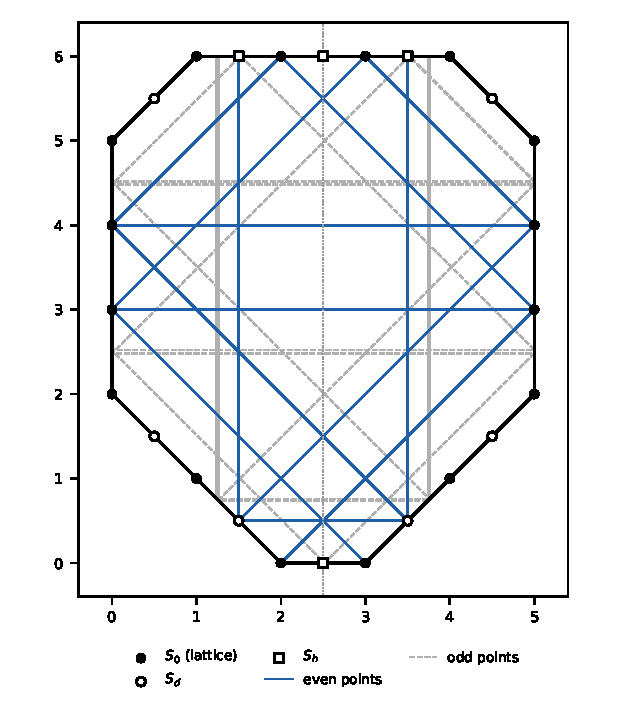
\includegraphics[width=.42\textwidth]{octagon-figure.pdf}
 \caption{The special octagon $O(5,6,1,2)$, which has the periods of~\cite[Figure~23]{ABS25}. Markers show the set $S$. The solid path joins the even points of the trajectory with $x_0=(2,0)$ and $x_1$ on the lower right diagonal side at parameter $37/100$; it ends at the vertex $(3,0)$ after $46$ steps. The even points include $(7/2,1/2)\in S_d$ and $(7/2,6)\in S_h$. Whenever an even point lies in $S_h$, the next odd point is on a vertical side. The dotted line is the axis of symmetry.}
 \label{fig:octagon}
\end{figure}

\begin{lemma}[half-lattice lemma]\label{lem:half}
Let $(x_0,x_1,\dots,x_{2m})$ be a trajectory in $O$ with $x_0\in V$. Then for every $0\le l\le m$:
\begin{enumerate}
\item[(a)] $x_{2l}\in S$;
\item[(b)] if $l<m$ and $x_{2l}\in S_h$, then $x_{2l+1}$ lies on a vertical side.
\end{enumerate}
\end{lemma}

\begin{proof}
Two facts are used. First, if $p\in\partial O$ is not on a horizontal side, then $\sigma_{(1,0)}(p)=\rho(p)$. Indeed $\rho(p)$ lies on the horizontal line through $p$, and $\rho(p)\ne p$ because $\partial O$ meets the axis $x=W/2$ only on the horizontal sides. In particular $\sigma_{(1,0)}$ maps each vertical side onto the other. Second, a chord through the interior cannot end on a side parallel to it, since it would then run along that side.

For $l=0$, $x_0\in V\subset S_0$, and (b) holds because no point of $S_h$ is a vertex. Assume (a) and (b) for some $l<m$. Put $p=x_{2l}$, $q=x_{2l+2}$ and let $d$ be the direction of $\side(x_{2l+1})$, so that $q=\sigma_d(p)$; if $p\notin V$, then $d$ is not parallel to $\side(p)$. We use~\eqref{eq:lines} throughout.

\emph{Case $p\in S_0$.} If $d$ is horizontal, then $p$ is not on a horizontal side and $q=\rho(p)\in\Z^2$. If $d$ is vertical, $q$ has the integer abscissa of $p$ and lies on a horizontal side or a diagonal side; in both cases $q\in\Z^2$. If $d=(1,\pm1)$, the chord preserves $k=x\mp y\in\Z$. If $q$ lies on a horizontal or vertical side, one coordinate of $q$ is an integer, hence both are. Otherwise $q$ lies on a diagonal side not parallel to $d$, on a line $x\pm y=K$ with $K\in\Z$, so $x(q)=(K+k)/2$ and $y(q)=\pm(K-k)/2$. Thus $q\in S_0\cup S_d$.

\emph{Case $p\in S_d$.} Both coordinates of $p$ lie in $\Z+\frac12$, so $x(p)\pm y(p)\in\Z$. If $d$ is horizontal, $q=\rho(p)$ lies on the mirror diagonal side and $x(q)=W-x(p)\in\Z+\frac12$, so $q\in S_d$. If $d$ is vertical, $x(q)=x(p)\in\Z+\frac12$; then $q\in S_h$ if $q$ is on a horizontal side, and $q\in S_d$ if $q$ is on a diagonal side, where $y(q)=\pm x(q)+K$. If $d$ is diagonal, it is not parallel to $\side(p)$, and the chord preserves one of the integers $x\pm y$. As in the previous case, $q\in S_0$ if $q$ is on a horizontal or vertical side and $q\in S_0\cup S_d$ otherwise. Thus $q\in S$, and $q\in S_h$ only if $d$ is vertical.

\emph{Case $p\in S_h$.} By (b), $x_{2l+1}$ is on a vertical side, so $d$ is vertical and $x(q)=x(p)\in\Z+\frac12$. Hence $q\in S_h$ if $q$ is on the other horizontal side and $q\in S_d$ otherwise. Again $q\in S_h$ only if $d$ is vertical.

This proves (a) for $l+1$. For (b), suppose $l+1<m$ and $q\in S_h$. The case analysis shows that $d$ is vertical, so $x_{2l+1}$ lies on a vertical side. Since $q$ lies on a horizontal side, $x_{2l+3}=\sigma_{(1,0)}(x_{2l+1})=\rho(x_{2l+1})$, which lies on the other vertical side.
\end{proof}

\begin{proof}[Proof of Theorem~\ref{thm:main}]
By Lemma~\ref{lem:normal} and affine invariance we may take the table to be $O=O(W,H,c_1,c_2)$. Every point of the critical set is an even point $x_{2l}$ of a trajectory starting at a vertex, so Lemma~\ref{lem:half} gives $C\subset S$. In particular $|C|\le|S|=N$. Theorem~\ref{thm:criterion} shows that every orbit is periodic with period at most $4(|C|^2-|C|)\le4(N^2-N)$.
\end{proof}

\begin{remark}\label{rem:rational}
A dilation of a lattice polygon by a rational factor is an affine image of a lattice polygon. Hence Theorem~\ref{thm:main} applies to every octagon with side slopes $0,\pm1,\infty$ and a vertical axis of symmetry whose width, height and two leg lengths (in the normal form of Lemma~\ref{lem:normal}) are rationally commensurable. The case of incommensurable real parameters is not covered.
\end{remark}

The same argument settles the mirror-symmetric part of the companion Hexhouse conjecture~\cite[Conjecture~6.1]{ABS25}. Following~\cite[Section~6]{ABS25} and their figures, a \emph{Hexhouse} is the lattice hexagon $X(s,h,p,q)$ with vertices $(0,0),(s,0),(s,s),(q,s+h),(p,s+h),(0,s)$, where $s,h,p,q$ are integers with $h>0$ and $0<p<q<s$: a square with a trapezoid on top. Up to scaling this has three integer parameters, as in~\cite{ABS25}. The Hexhouse drawn in~\cite[Figure~15]{ABS25} is not mirror symmetric; the one in~\cite[Figure~18]{ABS25}, with periods $4,44,68,92$, looks symmetric, and $X(3,1,1,2)$ has exactly these generic periods.

\begin{corollary}\label{cor:hex}
If $p+q=s$, every orbit in the Hexhouse $X(s,h,p,q)$ is periodic, with period at most $4(N^2-N)$, where $N=4hs+2ps$.
\end{corollary}

\begin{proof}
The linear map $(x,y)\mapsto(hx,py)$ sends $X(s,h,p,s-p)$ to the hexagon with vertices $(0,0),(hs,0),(hs,ps),(hq,ps+ph),(hp,ps+ph),(0,ps)$, which is $O(W,H,c_1,0)$ with $W=hs$, $H=p(s+h)$ and $c_1=hp$. These are integers with $2c_1<W$ (since $p<q=s-p$) and $c_1<H$. Lemma~\ref{lem:half} gives $C\subset S$ with $|S|=4W+2H-2c_1=4hs+2ps$, and Theorem~\ref{thm:criterion} applies.
\end{proof}

An affine map acts on directions by a projective transformation of the projective line, so it preserves the cross-ratio of four side directions. The directions $0,\infty,1,-1$ of $O(W,H,c_1,c_2)$ have cross-ratio $-1$, while the four side directions of $X(s,h,p,q)$, with slopes $0$, $\infty$, $h/p$ and $-h/(s-q)$, have cross-ratio $-1$ only when $p=s-q$. (An affine map preserves parallelism, so it must send the two parallel pairs of sides of $X(s,h,p,q)$, of slopes $0$ and $\infty$, to the two parallel pairs of $O(W,H,c_1,0)$, also of slopes $0$ and $\infty$; the cross-ratio of the ordered quadruple $(0,\infty;h/p,-h/(s-q))$ is $-(s-q)/p$ and must equal $-1$.) So Corollary~\ref{cor:hex} covers exactly the Hexhouses that are affine images of the hexagons $O(W,H,c_1,0)$, and the general case of~\cite[Conjecture~6.1]{ABS25} remains open.

\begin{remark}\label{rem:sharp}
Both hypotheses enter the proof. The lattice condition makes the constants in~\eqref{eq:lines} integers. The symmetry makes horizontal chords act as the reflection $\rho$, which keeps half-integer heights off the vertical sides and supplies clause~(b). Without~(b), a diagonal chord from a point of $S_h$ can reach a diagonal side at a point with quarter-integer coordinates; in $O(9,3,1,1)$ the chord of slope $1$ through $(\frac72,3)$ ends at $(\frac34,\frac14)$. The hypothesis of~\cite[Theorem~3.1]{ALW26}, finiteness of the set generated from the vertices by chords in \emph{all} side directions, holds for $O(3,3,1,1)$ and $O(4,4,1,1)$, where the set consists of the vertices. For $O(5,6,1,2)$, $O(6,5,2,1)$ and $O(7,9,3,2)$ the exploration has not closed after $20000$ points, which already have denominators up to $2^{14}$ or $2^{17}$. We do not prove that this set is infinite; the point is only that the filled-set criterion does not currently supply a proof for the family, whereas Lemma~\ref{lem:half} does.
\end{remark}

The symmetry hypothesis cannot simply be dropped.

\begin{proposition}\label{prop:asym}
Let $Q$ be the lattice octagon with vertices
\[(1,0),\ (3,0),\ (4,1),\ (4,4),\ (3,5),\ (2,5),\ (0,3),\ (0,1).\] Its opposite sides are parallel with slopes $0,\pm1,\infty$, it has no axis of symmetry, and not every orbit of its symplectic billiard map is periodic.
\end{proposition}

\begin{proof}
A reflection preserving $Q$ maps sides to sides of equal length. The horizontal and vertical sides have integer lengths and the diagonal sides have lengths in $\sqrt2\,\Z$, so the reflection preserves the pair of directions $\{0,\infty\}$, and its axis is horizontal, vertical or of slope $\pm1$. The cut corners have legs $1,1$ at the bottom and $1,2$ at the top, legs $1,2$ on the left, and the bounding box is $4\times5$, so none of these occurs. The points
\[
x_0=(4,\tfrac{11}3),\ x_1=(\tfrac53,0),\ x_2=(\tfrac23,\tfrac{11}3),\ x_3=(4,\tfrac73),\ x_4=(\tfrac23,\tfrac13),\ x_5=(\tfrac53,\tfrac{14}3)
\]
lie in the relative interiors of sides and form a $6$-periodic trajectory. Indeed, each chord $x_{k-1}x_{k+1}$ (indices mod $6$) is parallel to the side containing $x_k$ and passes through the interior. In the edge parameters $t_0,t_1$ of the sides of $x_0$ and $x_1$, the map $T^6$ is affine near $(x_0,x_1)$ with linear part $(t_0,t_1)\mapsto(-2t_0,-\frac12t_1)$; each factor is a product of three ratios of determinants of side vectors. Concretely, the even points are carried by the horizontal, vertical and slope-$1$ projections $x_0\mapsto x_2\mapsto x_4\mapsto x_6$, and a displacement $e$ of $x_0=(4,\frac{11}3)$ along its side returns as $-2e$; likewise a displacement $e$ of $x_1$ returns as $-\frac12e$. Since all six points lie in relative interiors of sides, this affine formula holds on a neighbourhood $U$ of $(x_0,x_1)$.

Let $q_s=(x_0,x_1+s)$, where $x_1+s$ denotes the point at signed distance $s$ from $x_1$ on its side, and $0<|s|$ is small. Then $T^{6k}(q_s)=(x_0,x_1+(-\frac12)^ks)\in U$ for all $k\ge0$, so the forward orbit of $q_s$ is defined, converges to $(x_0,x_1)$ and never reaches it. A periodic orbit is finite, so $q_s$ is not periodic.

It remains to show that the backward orbit of $q_s$ is defined for all but countably many $s$. It is the reversal of the forward trajectory $(y_k)_{k\ge0}$ with $y_0=x_1+s$ and $y_1=x_0$. By induction on $k$, the parameter interval splits into finitely many open intervals, on each of which $y_0,\dots,y_k$ are defined, their sides are fixed, each even point $y_{2l}$ is an injective affine function of $s$, and each odd point $y_{2l+1}$ is independent of $s$; the excluded parameters are the finitely many values of $s$ at which some $y_{2l}$ is a vertex. No odd point is a vertex. Otherwise $(y_{2l+1},y_{2l},\dots,y_1)$ would be a trajectory starting at a vertex that reaches $x_0$ after $2l$ steps. But such a trajectory applies to a vertex only parallel projections along the four side directions onto side lines $y=K$, $x=K$, $x\pm y=K$ with integer $K$; these preserve the set of points with dyadic rational coordinates, while $x_0$ has $y$-coordinate $\frac{11}3$. Hence the backward orbit fails only for countably many $s$, and $\Phi$ contains uncountably many non-periodic points.
\end{proof}

\section{Computations}\label{sec:computations}

The supplied programs use exact rational arithmetic and the Python standard library. They compute the critical set by following, for every vertex $x_0$ and every side, all trajectories with $x_1$ in that open side. Each state is an even point together with an open interval of odd points; an interval is split wherever an odd point could be sent to a vertex. The exploration terminates exactly when $C$ is finite. The second program was written independently from the explicit side equations~\eqref{eq:lines}; it checks clauses (a) and (b) of Lemma~\ref{lem:half} at every state.

\begin{itemize}
\item For all $1484$ admissible parameter tuples $(W,H,c_1,c_2)$ with $W,H,c_1,c_2\le14$ (mirror images and rescaled copies are counted separately), both programs find $C$ finite and $C\subset S$; the second also confirms clause~(b). For the $340$ octagons with parameters at most $10$, a comparison script confirms that the two programs produce identical critical sets and identical numbers of explored states. The largest critical set has $58$ points.
\item A third, standard-library script verifies the trajectory and the multipliers $-2$ and $-\frac12$ of Proposition~\ref{prop:asym} from the side equations, including an exact perturbation test. In three further asymmetric lattice octagons the exploration of $C$ did not terminate within $40000$ states; a centrally symmetric one without a mirror axis had finite $C$.
\item The generic periods of $O(5,6,1,2)$ are $4,16,32,44,68,92$, the periods reported for the octagon of~\cite[Figure~23]{ABS25}. They were computed exactly from two off-centre rational points in every cell. The trajectory of Figure~\ref{fig:octagon} has $46$ steps, and $|C|=20$ for this octagon.
\end{itemize}

These checks test the lemma and its implementation. The theorem rests on the written proof.

\paragraph{The companion conjectures.} The same programs give checked computations for two other conjectures of~\cite{ABS25}. For each of the $1007$ Hexhouses $X(s,h,p,q)$ with integer parameters $s,h,p,q\le11$, up to scaling and mirror image, the critical set is finite (the largest has $|C|=205$); by Theorem~\ref{thm:criterion}, each of these Hexhouses is fully periodic. For the $252$ symmetric ones ($p+q=s$) a separate script confirms $C\subset S$ after the map of Corollary~\ref{cor:hex}. For a grid of $60$ rational Penthouses (a unit square with apex $(b,1+a)$) with moduli $m=\lfloor(a+1)/a\rfloor$ from $1$ to $7$, the critical set is finite and the generic periods are exactly $16m-4$, $16m+4$ and $16m+12$, as Conjecture~4.1 of~\cite{ABS25} predicts. These instances do not prove Conjecture~6.1 or Conjecture~4.1 of~\cite{ABS25}, which concern infinite families.

\paragraph{Beyond the lattice.} In exploratory runs, octagons with slopes $0,\pm1,\infty$ and a vertical axis of symmetry, but with generic rational legs of denominator $10007$, also had finite critical sets (six of six instances, with up to $582$ points). Generic real Hexhouses behaved the same way, whereas a square with a generic two-vertex cap did not. Lemma~\ref{lem:half} uses the lattice essentially, so full periodicity of the real families is left open.

\section{Scope}

Theorem~\ref{thm:main} settles Conjecture~6.2 of~\cite{ABS25}, and Corollary~\ref{cor:hex} settles the mirror-symmetric case of Conjecture~6.1. The criterion of Section~\ref{sec:criterion} is due to Albers, Lander and Westermann~\cite{ALW26}; the contribution here is Lemma~\ref{lem:half} and its consequences, Theorem~\ref{thm:main} and Corollary~\ref{cor:hex}. The Hexhouse conjecture for Hexhouses without mirror symmetry, the Penthouse conjecture, and the existence of a single convex polygon without periodic symplectic billiard orbits~\cite[Question~7.1]{ABS25},~\cite{ALW26} remain open. The period bound is far from the observed periods, and the exact period sets of special octagons are not determined here.

\paragraph{Research assistance.}
Valyu Search and DeepResearch located the sources and searched for later work. Coding agents ran the exact experiments that suggested the half-lattice invariant, wrote the verification programs and drafted this manuscript. An independent referee report on this package found no gap in the proofs, with high confidence in the theorem and moderate confidence in novelty. Internal reviews are not external peer review; what a reader can verify is the written proof and the programs in \path{verification/}.

\smallskip
\noindent\textbf{Reproduction.} From this directory, run \texttt{sh build.sh}. It replays both verification programs, the companion-family checks and the figure, then builds this paper. The programs and saved results are in \path{verification/}.

\bibliographystyle{plain}
\bibliography{references}
\end{document}
